\documentclass[10pt,a4paper]{article}
\input{AEDmacros}
\usepackage{etoolbox}
\usepackage{adjustbox}
\usepackage{inconsolata}
\usepackage{tcolorbox}
\usepackage{xcolor}
\usepackage{ragged2e}
\usepackage{changepage}
\usepackage{amssymb}
\usepackage[outputdir=out]{minted}
\DeclareRobustCommand{\ttfamily}{\fontencoding{T1}\fontfamily{lmtt}\selectfont}

\lstset{
  basicstyle=\ttfamily,
  numbers=none,
  frame=none,
  xleftmargin=10px,
  aboveskip=0pt
}
\newcommand{\vacio}{\emptyset}
\newcommand{\limn}{\lim_{n \to \infty}}
\newcommand{\ceil}[1]{%
  \left\lceil #1 \right\rceil%
}
\newcommand{\reales}{\mathbb{R}}
\newcommand{\limite}[2]{%
  \lim_{#1 \to #2}
}

\newenvironment{groupIzq}[1]{%
  \begin{list}{}{%
      \setlength{\leftmargin}{#1}%
      \setlength{\topsep}{0pt} % Elimina el espacio superior
      \setlength{\partopsep}{0pt} % Asegura que no haya espacio extra
    }
  \item[]
}{%
  \end{list}
}
\newcommand{\demoline}{\vspace{0.5em}}

\newcommand{\Indent}{\hspace*{0.75cm}}
\newcommand{\MiniIndent}{\hspace*{0.325cm}}
\newcommand{\Int}{\ensuremath{int}}

\newcommand{\Extends}[2]{%
  \noindent\ensuremath{\texttt{\textbf{#1}}\ \texttt{\textbf{extends}}\ #2}%
  \par
}
\newcommand{\Array}[1]{\ensuremath{Array \texttt{<}#1\texttt{>}}}
\newcommand{\Tupla}[1]{\ensuremath{Tupla \texttt{<}#1\texttt{>}}}
\newcommand{\Tuple}[1]{\ensuremath{Tuple \texttt{<}#1\texttt{>}}}
\newcommand{\Clase}[2]{\texttt{#1<#2>}}
\newcommand{\Type}[2]{%
  \noindent\ensuremath{\texttt{\textbf{#1}} = #2}%
  \par
}
\newcommand{\primitiva}[1]{\ensuremath{#1}}
\newcommand{\Arr}[1]{\ensuremath{Array \langle #1 \rangle}}
\newcommand{\conj}[1]{\ensuremath{conj \langle #1 \rangle}}
\newcommand{\union}{\cup}
\newcommand{\interseccion}{\cap}
\newcommand{\Struct}[1]{\ensuremath{\texttt{Struct} \langle \texttt{#1} \rangle}}
\newcommand{\StructField}[2]{\normalfont\ttfamily{#1}: \ensuremath{#2}}
\newcommand{\Title}[1]{%
  \raggedright
  \noindent{\textbf{#1}}%
  \justifying
  \vspace{1em}%
}

\newcommand{\TitlePar}[1]{%
  \raggedright
  \noindent{\textbf{#1}}%
  \justifying%
}

\newcommand{\Var}[2]{%
  \noindent\texttt{var \textbf{#1}}: #2 \par
}
\newenvironment{Vars}{%
  \begin{flushleft} % Alineación a la izquierda
}{%
  \end{flushleft}
  \vspace{1em} % Salto de línea final
}

\newenvironment{ModuloImplements}[2]{%
  \raggedright
  \texttt{Modulo #1\ implements\ #2\ \{}
  \justifying
  \begin{adjustwidth}{2em}{0em}
}{%
  \end{adjustwidth}
  \texttt{\}}%
}

\definecolor{lightgray}{gray}{1}
\definecolor{darkgray}{gray}{0.65}
\newcommand{\comentario}[1]{%
  \noindent{\normalfont\bfseries\ttfamily\small\textcolor{darkgray}{\% #1\ \ \%} \par}%
}

\newtcolorbox{ImplementationCodeBoxFixedWithParam}[1]{colback=lightgray!20, colframe=white, boxrule=0pt, left=5pt, right=5pt, top=5pt, bottom=5pt, width=#1}
\newtcolorbox{ImplementationCodeBoxFixed}{colback=lightgray!20, colframe=white, boxrule=0pt, left=5pt, right=5pt, top=5pt, bottom=5pt, width=0.8\linewidth}
\newtcolorbox{ImplementationCodeBox}{colback=lightgray!20, colframe=white, boxrule=0pt, left=5pt, right=5pt, top=5pt, bottom=5pt, width=\dimexpr\textwidth-2em\relax}
\definecolor{lightgray}{RGB}{220,220,220}
\newenvironment{ImplementationCode}[1]{%
  \VerbatimEnvironment
  \vspace{-0.2em}
  \begin{ImplementationCodeBoxFixedWithParam}{#1}
  \flushleft
  \begin{adjustbox}{minipage=\dimexpr\textwidth-2em\relax, margin=0pt}
  \begin{minted}[linenos, xleftmargin=-2.4em, numbersep=-2.5em]{java}%
}{
  \end{minted}
  \end{adjustbox}
  \vspace{-0.25em}
  \end{ImplementationCodeBoxFixedWithParam}
  \fussy
}

\usepackage{graphicx}
\usepackage{svg}
\setsvg{inkscape=/Applications/Inkscape.app/Contents/MacOS/inkscape}

\graphicspath{{images/}}

\geometry{paperwidth=21cm, paperheight=80cm}

\begin{document}

\Title{Ejercicio Parcial Mediciones}

\begin{figure}[h]
  \centering
  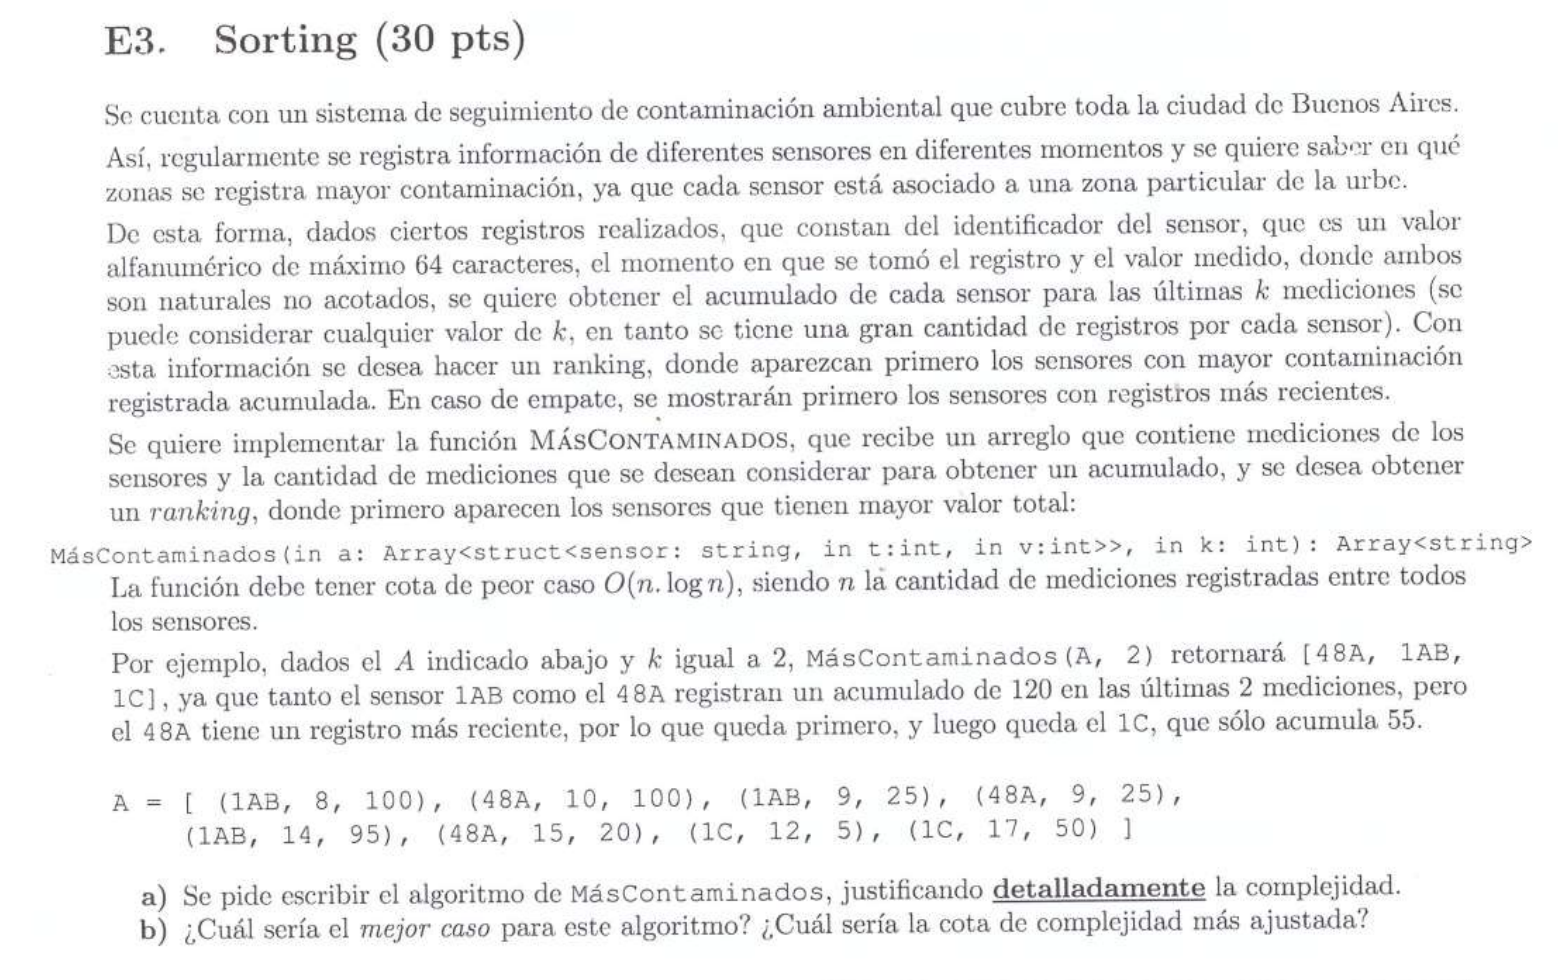
\includegraphics[width=\textwidth]{images/mediciones.png}
  \caption{Enunciado Mediciones}
  \label{fig:mediciones}
\end{figure}

\Type{SensorId}{string}
\Type{Sensor}{\Struct{\StructField{sensor}{SensorId}, \StructField{t}{int}, \StructField{v}{int}}}
\Type{Medicion}{\Struct{\StructField{sensorId}{SensorId}, \StructField{t}{int}, \StructField{valorAcmulado}{int}, \StructField{mediciones}{int}}}

\begin{proc}{MasContaminados}{\In A: \Clase{Array}{Sensor}, \In k: int}{\Clase{Array}{SensorId}}
  \begin{ImplementationCode}{470px}
      mergeSort(A) // Ordenar por mas recientes "t" mayor a menor. O(n*log(n))

      // El diccionario digital funciona en O(1)
      // por el largo maximo es de 64 caracteres
      // y el alfabeto está acotado.
      var mediciones: DiccionarioDigital<SensorId, Medicion>
      var sensores: ListaEnlazada<SensorId>
          mediciones:= diccionarioVacio()
          sensores:= listaVacia()

      var j: int
          j:= 0

      while (j < A.length) do // O(n)
        var sensorId: SensorId
            sensorId:= A[j].sensor

        if (!mediciones.esta(sensorId)) then
          // Nos quedamos con la fecha mas reciente
          mediciones.definir( // O(1)
            sensorId,
            new Medicion(
              sensorId=sensorId,
              mediciones=1
              t=A[j].t
              valorAcumlado=A[j].v,
            ) // O(1)
            sensores.agregarAtras(sensorId)
          )
        else
          var medicion: Medicion
              medicion:= sensores.obtener(sensorId) // O(1)

          if (medicion.mediciones < k) then
            medicion.mediciones:= medicion.mediciones + 1 // O(1)
            medicion.valorAcumulado:= medicion.valorAcumulado + A[j].v // O(1)
            // Nos vamos quedando con la fecha mas reciente dentro de las "k" mediciones
            medicion.t:= A[j].t // O(1)
          endif
        endif
      endwhile

      // Ahora que tenemos el diccionario armado, con los ultimos "k" valores
      // acumulados, solo tenemos que pasarlo a un array y ordenarlo primero
      // por el desempate (t menor a mayor) y luego por valorAcmulado (mayor a menor)
      var resultadoMedicionesLista: ListaEnlazada<Medicion>
      var resultadoMediciones: Array<Medicion>

      while !(sensores.vacia()) do // O(n)
        resultadoMedicionesLista.agregarAtras(mediciones.obtener(sensores.primero())) // O(1)
        sensores.fin() // O(1)
      endwhile

      resultadoMediciones:= toArray(resultadoMediciones) // O(n)
      
      mergeSort(resultadoMediciones) // ordenar por "t" menor a mayor O(n*log(n))
      mergeSort(resultadoMediciones) // ordenar por "valorAcumulado" mayor a menor O(n*log(n))

      var res: Array<SensorId>
          res:= new Array(resultadoMediciones.length) // O(n)
          j:= 0 // O(1)

      while (j < res.length) do // O(n)
        res[j]:= resultadoMediciones[j].sensorId
      endwhile

      return res
      /**
      * Analisis complejidad: O(n*log(n))
      */
  \end{ImplementationCode}
\end{proc}


\newpage

\Title{Ejercicio 14}

\par Para poder resolver este problema con la complejidad que nos piden vamos
\par a tener que utilizar una combinacion entre heap sort y listas enlazadas.
\par Fijémonos por qué merge no sirve:
\par Supongamos que tenemos el arreglo [2,3,4] y k=2
\par Si pudieramos armar el siguiente arreglo en n*k: [2, 4, 3, 6, 4, 8]
\par Nos damos cuenta que podríamos ir haciendo merge de a partes.
\par Paso 1: merge([2,4], [3,6]) \ensuremath{-->} [2,3,4,6]
\par Paso 2: merge([2,3,4,6], [4, 8]) \ensuremath{-->} [2,3,4,4,6,8]
\par Esto no funciona, la complejidad de hacer merge en n listas ordenadas es cuadratica.
\par (es una sumatoria de gauss)
\par Así que: Heap sort al rescate. Vamos a usar listas enlazadas para que remover el primero sea O(1)

\begin{proc}{ordenarMultiplos}{\In A: \Clase{Array}{int}, \In k: int}{\Clase{Array}{int}}
  \begin{ImplementationCode}{470px}
      var res: Array<int>
          res:= new Array(A.length * k) // O(n*k)

      var arregloDeListas: Array<ListaEnlazada<int>>
          arregloDeListas:= new Array(A.length)
      var j: int
      var i: int
          i:= 1
          j:= 0

      while (j < A.length) do
        arregloDeListas[j] = listaVacia()

        while (i <= k) do
          arregloDeListas[j].agregarAtras(A[j] * i)
          i:= i + 1
        endwhile

        i:= 1
        j:= j + 1
      endwhile

      // Cola de prioridad min, por el primer elemento de la lista enlazada
      var colaDePrioridad: ColaDePrioridadLog<ListaEnlazada<int>>
          colaDePrioridad:= colaDePriodidadVacia()
          j:= 0

      while (j < arregloDeListas.length) do
        colaDePrioridad.encolar(arregloDeListas[j])
        j:= j + 1
      endwhile

      var res: Array<int>
      var indiceActual: int
          res:= new Array(A.length * k)
          indiceActual:= 0

      while (!colaDePriodidad.estaVacia())
        var listaPrioritaria: ListaEnlazada<int>
            listaPrioritaria:= colaDePriodidad.desencolarMax()
        
        res[i]:= listaEnlazada(listaPrioritaria.primero())

        listaPrioritaria.fin()
        colaDePriodidad.encolar(listaPrioritaria)

        i:= i + 1
      endwhile

      return res
  \end{ImplementationCode}
\end{proc}
\newpage

\Title{Ejercicio 17}

\Type{Planta}{string}
\Type{Stock}{int}
\Type{Prioridad}{int}
\Type{Nodo}{\Struct{\StructField{planta}{Planta}, \StructField{stock}{Stock}, \StructField{prioridad}{Prioridad}}}

\begin{proc}{Recolectar}{
  \\\Indent\In s: \Clase{Array}{\Clase{Tupla}{Planta, Stock}},
  \\\Indent\In u: \Clase{DiccionarioDigital}{Planta, Prioridad}
\\}{\Clase{Array}{Planta}}
  \begin{ImplementationCode}{470px}
      var stockTotal: DiccionarioDigital<Planta, Stock>
          stockTotal:= diccionarioVacio()
    
      // Inicializamos stockTotal
      var j:= 0
      while (j < s.length) do
        var planta: Planta
        var stock: Stock
        var stockAcumulado: Stock
            planta:= s[j][0]
            stock:= s[j][1]
            stockAcumulado:= 0
    
        if (stockTotal.pertenece(planta)) then
            stockAcumulado:= stockTotal.obtener(planta)
        endif
    
        stockTotal.definir(Planta, stockAcumulado + stock)
        j:= j + 1
      endwhile
    
      // Evitemos a toda costa iterar sobre un dict
      // justificar que se amortiza es siempre complicado
      // TRUCAZO
      var nodos: ListaEnlazada<Nodo>
          nodos:= listaVacia()
          j:= 0
    
      while (j < s.length) do
        var planta: Planta
            planta:= s[j][0]
        if (stockTotal.pertenece(planta)) then
          var prioridad: Prioridad
          var stock: Stock
              prioridad:= u.obtener(planta)
              stock:= stockTotal.obtener(planta)
    
          nodos.agregarAtras(new Nodo(planta=planta, stock=stock, prioridad=prioridad))
          stockTotal.borrar(planta)
        endif
        j+= j + 1
      endwhile
    
      var arreglo_nodos: Array<Nodo>
          arreglo_nodos:= toArray(nodos)
      
      mergeSort(arreglo_nodos) // ordenar de menor a mayor por stock
      mergeSort(arreglo_nodos) // ordenar de mayor a menor por prioridad
    
    
      var res: Array<Planta>
          res:= new Array(arreglo_nodos.longitud())
          j:=0
    
      while (j < arreglo_nodos.longitud()) do
        res[j]:= arreglo_nodos[j].planta
        j:= j + 1
      endwhile
    
      return res
  \end{ImplementationCode}
\end{proc}

\newpage
\Title{Ejercicio 18}

\Type{Libreta}{int}
\Type{Nota}{int}
\Type{Promedio}{float}
\Type{Contador}{\StructField{totalNotas}{int}, \StructField{notasAcumuladas}{Nota}}

\begin{proc}{OrdenarPorLibretaYPromedios}{\In s: \Clase{Array}{\Clase{Tupla}{Libreta, Nota}}}{\Clase{Array}{\Clase{Tupla}{Libreta, Promedio}}}
  \begin{ImplementationCode}{470px}
      var promedios: DiccionarioDigital<Libreta, Contador>
      promedios:= diccionarioVacio()

      var j: int
          j:= 0

      // Inicializamos el dict.
      while (j < s.length) do
        var libreta: Libreta
            libreta:= s[j][0]
        promedios.definir(
          libreta,
          new Contador(s[j], new Contador(totalNotas=0, notasAcumuladas=0))
        )
        j += 1
      endwhile

      // Insertamos las notas acumuladas.
      j:= 0
      while (j < s.length) do
        var libreta: Libreta, nota: Nota
            libreta:= s[j][0], nota:= s[j][1]

        var contador: contador
            contador:= promedios.obtener(libreta)

        contador.totalNotas:= contador.totalNotas + 1
        contador.notasAcumuladas:= nota

        // No hace falta re-definir, hay aliasing
        j += 1
      endwhile

      // Creamos res
      var res: Array<Tupla<Libreta, Promedio>>
          res:= new Array<promedios.tamaño()

      // Vamos a zafar de iterar promedios, nunca queremos
      // iterar y tener que justificar que las operaciones
      // se amortizan, TRUCAZO:
      var i: int
          i:= 0
          j:= 0
      while (j < s.length) do
        var notaAcumulada: Nota
        var libreta: Libreta
            nota:= s[j][1]
            libreta:= s[j][0]
      
        if (promedios.pertenece(libreta))
          var contador: contador
              contador:= promedios.obtener(libreta)

          res[i]:= <libreta, contador.notasAcumuladas / contador.totalNotas>
          promedios.borrar(libreta)

          i:= i + 1
        endif

        j:= j + 1
      endwhile

      mergeSort(res) // ordenar res por la primera coordenada: libreta. (menor a mayor)
      mergeSort(res) // ordenar res por la segunda coordenada: promedio. (mayor a menor)

      return res
  \end{ImplementationCode}
\end{proc}

\newpage
\Title{Ejercicio 19}

\Type{Prioridad}{int}
\Type{Nodo}{\Struct{\StructField{prioridad}{Prioridad}, \StructField{valor}{int}}}

\begin{proc}{OrdenarSegunCriterio}{\In s: \Clase{Array}{int}, \In crit: \Clase{Array}{Prioridad}}{\Clase{Array}{int}}
  \begin{ImplementationCode}{470px}
      var s1: ListaEnlazada<Nodo>
      var s2: ListaEnlazada<int>
      var critDict: DiccionarioLog<int, Prioridad>
          s1:= listaVacia()
          s2:= listaVacia()
          critDict:= diccionarioVacio()
      
      var prioridad: int
          prioridad:= 0
      
      // Inidicalizamos crit dict.
      while (prioridad < crit.length) do
        critDict.definir(crit[prioridad], prioridad)
        prioridad:= prioridad + 1
      endwhile
    
      var j: int
          j:= 0
      
      // Insertamos en las listas s1 y s2.
      while (j < s.length) do
        if critDict.pertenece(s[j]) then
          s1.agregarAtras(s[j], new Nodo(prioridad=critDict.obtener(s[j]), valor=s[j])
        else
          s2.agregarAtras(s[j])
        endif
      endwhile
    
      // Ordenar la primera parte del arreglo
      var s1Arreglo: Array<Nodo>
      var s1Valores: Array<int>
          s1Arreglo:= toArray(s1)
          s1Valores:= new Array(s1Arreglo.length)
    
      mergeSort(s1Arreglo) // ordenar s1Arreglo por prioridad.
      // No hay criterio de desempate pues crit no tiene repetidos
    
      j:= 0
      while (j < s1Arreglo.length) do
        s1Valores[j]:= s1Arreglo[j].valor
        j:= j + 1
      endwhile 
    
      // Ordenar la segunda parte del arrego
      var s2Valores: Array<int>
          s2Valores:= toArray(s2)
    
      mergeSort(s2Valores) // ordenar s2Arreglo de menor a mayor
    
      // Concatenar en res.
      var res: Array<int>
          res:= concat(s1Valores, s2Valores)
    
      // Devolver res.
      return res
  \end{ImplementationCode}
\end{proc}

\end{document}